\documentclass{book}

\usepackage[a4paper,top=2.0cm,bottom=2.0cm,left=2.0cm,right=2.0cm]{geometry}

%\documentclass[pdftex,10pt,a4paper]{book}
%\usepackage[paperwidth=19cm,
%paperheight=26cm, outer=2cm, 
%top=1.5cm, bottom=1.5cm]{ geometry}

\usepackage[english,italian]{babel} %l'ultima lingua è quella che legge per i titoli
\usepackage[utf8]{inputenc}
\usepackage[T1]{fontenc,url}
\usepackage{titlesec}
\usepackage{easylist}
\usepackage{hanging}

\usepackage[pdftex,colorlinks]{hyperref}
\hypersetup{
	colorlinks=true,
	linkcolor=black,
	filecolor=magenta,
	urlcolor=cyan,
}
\usepackage{hypcap}
\usepackage{blindtext}
\usepackage{tipa}
\usepackage{epigraph}
\usepackage{enumerate}
\usepackage{longtable}
\usepackage{setspace}
\usepackage{verbatim}
\usepackage{graphicx}
\usepackage{amsmath}
\usepackage{pbox}
\usepackage{fancyhdr}
\usepackage{cancel}
\usepackage{tabularx}
\usepackage{booktabs}
\usepackage{multirow}
\usepackage{longtable}
\usepackage{tikz}
\usepackage{tikz-qtree}
\usepackage{subfig}
\usepackage{xcolor}
\usepackage{amssymb}
\usepackage{amsmath}
\usepackage{mathrsfs}
\usepackage{textcomp}
\usepackage{circuitikz}
\usepackage{pifont}
\usepackage{imakeidx}
\usepackage{verbatim}
\usepackage{dsfont}
\usepackage{listings}
\usepackage{color}
\usepackage{upgreek}
\usepackage{tasks}
\usepackage{exsheets}
\usepackage{pgfplots}
\usepackage{amsthm}


\usepackage{showframe}
\renewcommand\ShowFrameLinethickness{0.15pt}

\usepackage{matlab-prettifier}

\definecolor{mygreen}{rgb}{0,0.6,0}
\definecolor{mygray}{rgb}{0.5,0.5,0.5}
\definecolor{mymauve}{rgb}{0.58,0,0.82}

\lstset{ 
  backgroundcolor=\color{white},   % choose the background color; you must add \usepackage{color} or \usepackage{xcolor}; should come as last argument
  basicstyle=\footnotesize,        % the size of the fonts that are used for the code
  breakatwhitespace=false,         % sets if automatic breaks should only happen at whitespace
  breaklines=true,                 % sets automatic line breaking
  captionpos=b,                    % sets the caption-position to bottom
  commentstyle=\color{mygreen},    % comment style
  deletekeywords={...},            % if you want to delete keywords from the given language
  escapeinside={\%*}{*)},          % if you want to add LaTeX within your code
  extendedchars=true,              % lets you use non-ASCII characters; for 8-bits encodings only, does not work with UTF-8
  firstnumber=1000,                % start line enumeration with line 1000
  frame=single,	                   % adds a frame around the code
  keepspaces=true,                 % keeps spaces in text, useful for keeping indentation of code (possibly needs columns=flexible)
  keywordstyle=\color{blue},       % keyword style
  language=Octave,                 % the language of the code
  morekeywords={*,...},            % if you want to add more keywords to the set
  numbers=left,                    % where to put the line-numbers; possible values are (none, left, right)
  numbersep=5pt,                   % how far the line-numbers are from the code
  numberstyle=\tiny\color{mygray}, % the style that is used for the line-numbers
  rulecolor=\color{black},         % if not set, the frame-color may be changed on line-breaks within not-black text (e.g. comments (green here))
  showspaces=false,                % show spaces everywhere adding particular underscores; it overrides 'showstringspaces'
  showstringspaces=false,          % underline spaces within strings only
  showtabs=false,                  % show tabs within strings adding particular underscores
  stepnumber=2,                    % the step between two line-numbers. If it's 1, each line will be numbered
  stringstyle=\color{mymauve},     % string literal style
  tabsize=2,	                   % sets default tabsize to 2 spaces
  title=\lstname                   % show the filename of files included with \lstinputlisting; also try caption instead of title
}

\linespread{1.5} % l'interlinea

\newtheorem{defi}{Definizione}
\newtheorem{notab}{Nota Bene}
\newtheorem{oss}{Osservazione}

\frenchspacing

\newcommand{\abs}[1]{\lvert#1\rvert}

\usepackage{floatflt,epsfig}

\usepackage{multicol}
\newcommand\yellowbigsqcup[1][\displaystyle]{%
  \fboxrule0pt
  \ifx#1\textstyle\fboxsep-0.6pt\else\fboxsep-1.25pt\fi
  \mathrel{\fcolorbox{white}{yellow}{$#1\bigsqcup$}}}

\lstset{language=Octave,keywordstyle={\bfseries \color{red}}}

\title{Manuale base GNU/Octave}
\author{Nicola Ferru}
\begin{document}
\maketitle
\tableofcontents
\chapter{Introduzione}
\label{chap:intro}
\begin{defi}
  GNU/Octave è un applicativo per il calcolo matriciale che consente di svilgere
  tutte le operazioni base e non solo a riguardo, dallo somma, divisione,
  moltiplicazioni e sottrazioni tra matrici, calcolo del determinante, del
  grado e tanto altro.
\end{defi}

\section{Pacchetti e impostazioni base}
\label{sec:packbase}

\subsection{Pacchetti}
\label{sec:pack}

\begin{table}[th]
  \centering
  \begin{tabular}{ll}
    {\bf Nome} & {\bf Descrizione}\\\hline
    \href{https://gnu-octave.github.io/packages/fuzzy-logic-toolkit/}{fuzzy-logic-toolkit} & Un toolkit di logica fuzzy per lo più
                                                                                               compatibile con MATLAB per Octave \\\hline
    \href{https://gnu-octave.github.io/packages/symbolic/}{symbolic} & Aggiunge funzionalità di calcolo simbolico a GNU
                        Octave \\\hline
    \href{https://gnu-octave.github.io/packages/ocs/}{Circuit Simulator (OCS)} & Risolvere equazioni di circuiti elettrici DC e transitori. \\\hline
    \href{https://gnu-octave.github.io/packages/control/}{Control} & Strumenti CACSD ({\it Computer-Aided Control System
                       Design}) per GNU Octave,\\ &basati sulla libreria SLICOT.\\\hline
    \href{https://gnu-octave.github.io/packages/instrument-control/}{instrument-control} & Funzioni I/O di basso livello per interfacce seriali, i2c, parallele, tcp, gpib, vxi11,\\
               &udp e usbtmc.\\\hline 
  \end{tabular}
  \caption{pacchetti utili}
  \label{tab:pachutil}
\end{table}

\subsection{Funzione di identificazione di una variabile}
\label{sec:funiden}
\begin{table}[ht]
  \centering
  \begin{tabular}[tab:funzionediid]{ll}
    {\bf Nome} & {\bf Descrizione} \\\hline
    \lstinline|whos M| & stampa i dati completi sulla variabile
  \end{tabular}
  \caption{Funzione di identificazione}
  \label{tab:funzionediid}
\end{table}
\subsubsection{Stampa a video}
\label{sec:stampiden}
\begin{small}
\begin{verbatim}
Variables visible from the current scope:
variables in scope: top scope
  Attr   Name        Size                     Bytes  Class
  ====   ====        ====                     =====  =====
         M           3x3                         72  double
Total is 9 elements using 72 bytes
\end{verbatim}
\end{small}
\clearpage

\subsubsection{Come funziona}
All'interno di Octave e Matlab sono presenti le classi di variabili
esattamente come accade in altri linguaggi più di programmazione più blasonati,
esso ovviamente è relegato alle funzioni matematiche e grafiche per cui è
pensato il programma.
\begin{figure}[ht]
  \centering
  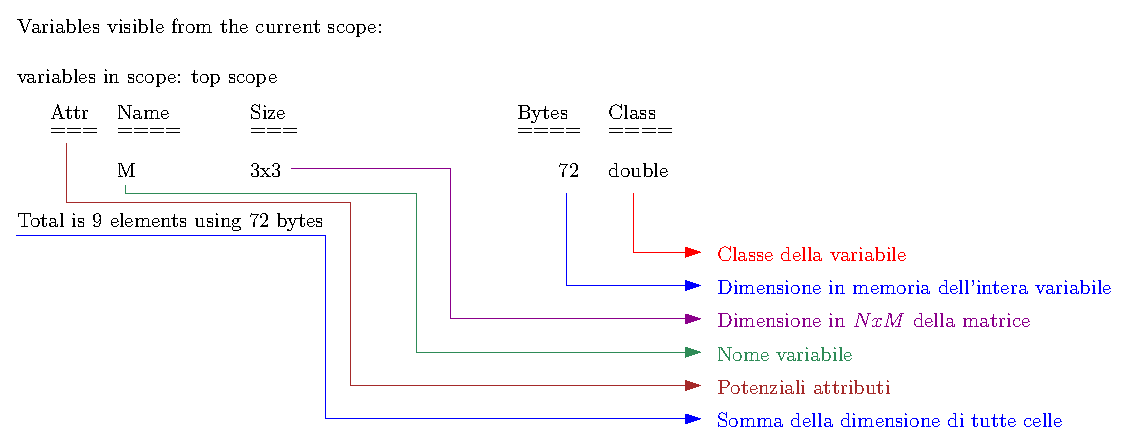
\includegraphics[width=15cm]{img/finiti/whos.eps}
  \caption{descrizione dell'interfaccia di funzione}
  \label{fig:interffun}
\end{figure}
\begin{notab}
  Anche la variabile singola viene vista come una matrice 1x1, da questo si
  denota che come il suo cugino Matlab è un software pensato per elaborare
  prodotti matriciali, infatti, il nome Matlab non sta per \texttt{Mathematic
    lab} ma per \texttt{Matrix Lab}. 
\end{notab}
\subsection{Tipi variabile}
\label{sec:tipivariabile}

\begin{table}[ht]
  \centering
  \begin{tabular}{llll}
    {\bf Nome} & {\bf Descrizione} & {\bf Dimensione} & {\bf Cifre rappresentabili}\\\hline
    \lstinline|double| ({\bf default}) & double-precision array & 8byte & $\pm1.79769x10^{308}$ a $\pm2.22507x10^{-308}$\\\hline
    \lstinline|single| & single-precision array & 4byte & $-2.1475x10^9$ a $2.1475x10^9$\\\hline 
    \lstinline|int8| & Array di interi con segno & 8bit & $-128$ a $127$\\\hline
    \lstinline|int16| & Array di interi con segno & 16bit & $-32768$ a $32767$ \\\hline
    \lstinline|int32| & Array di interi con segno & 32bit & $-2.1475x10^9$ a $2.1475x10^9$\\\hline 
    \lstinline|int64| & Array di interi con segno & 64bit & $-9.2234x10^{18}$ a $9.2234x10^{18}$\\\hline
    \lstinline|uint8| & Array di interi senza segno & 8bit & $255$\\\hline
    \lstinline|uint16| & Array di interi senza segno & 16bit & $65535$ \\\hline
    \lstinline|uint32| & Array di interi senza segno & 32bit & $4.2950x10^9$\\\hline 
    \lstinline|uint64| & Array di interi senza segno & 64bit & $1.8447x10^{19}$\\\hline
  \end{tabular}
  \caption{Tipi variabile}
  \label{tab:tipivariabile}
\end{table}
\begin{oss}
  Questa rapresentazione in memoria vale per la singola cella, quindi bisogna
  moltiplicare il paso per il numero di celle dello stesso tipo. Il programma
  peserà quanto il numero complessivo delle variabili presenti.
\end{oss}

\paragraph{Le stringhe --}
Un altro tipo di variabile però implicita sono le stringhe che il programma può
gestire, nel sequente modo \lstinline|str = "string x"| e la stampa di stringa
viene fatta con un semplice \lstinline|printf(str)|.
\clearpage
\subsubsection{Cosa stampa e cosa no}
Nel linguaggio di Matlab e Octave vengono stampate tutte le associazioni,
funzioni e inizializzazioni che non terminano con il ``{\color{red};}''.

\subsection{Impostazioni e formati}
\label{sec:formImp}
\begin{table}[ht]
  \centering
  \begin{tabular}{lll}
    {\bf Nome} & {\bf Descrizione} & {\bf Visuale}\\\hline
    \lstinline|rat| & Aspetto rateo (invece dei numeri reali rende numeri frazionari) & 1/2\\\hline
    \lstinline|short| & Formato breve a decimale fisso con 4 cifre dopo la virgola. (\textit{default}) & 0.5000\\\hline
    \lstinline|long| & Formato lungo a decimale fisso con 15 cifre dopo la virgola per & 0.500000000000000\\
                     &  i valori doppi e 7 cifre dopo la virgola per i valori singoli. \\\hline
    \lstinline|shortE| & Formato breve in annotazione scientiica con 4 cifre dopo la virgola & 5.0000e-01\\\hline
    \lstinline|longE| & Formato lungo a decimale fisso con 15 cifre dopo la virgola per & 5.000000000000000e-01\\
               & i valori doppi e 7 cifre dopo la virgola per i valori singoli.\\\hline
    \lstinline|shortG| & Formato breve, decimale fisso o notazione scientifica, a seconda & 0.5000\\ & di quale sia più compatto, con un totale di 5 cifre.\\\hline
    \lstinline|longG| & Formato lungo a decimali fissi o notazione scientifica, qualunque & 0.500000000000000\\
               & sia il più compatto, con un totale di 15 cifre per i valori doppi e\\ & 7 cifre per i valori singoli.\\\hline
    \lstinline|shortEng| & Breve notazione ingegneristica (l'esponente è un
                           multiplo & 500.0000e-003\\
    
               &di 3) con 4 cifre dopo la virgola.\\\hline
    \lstinline|longEng| & Notazione ingegneristica lunga (l'esponente è un multiplo di 3) & 500.000000000000000e-003\\ & con 15 cifre significative.\\\hline
    \lstinline|+|&Formato positivo/negativo con caratteri +, - e vuoti visualizzati & +\\
               & per elementi positivi, negativi e zero.\\\hline
    bank & Formato valuta con 2 cifre dopo la virgola. & 0.50 \\\hline
    hex & Rappresentazione esadecimale di un numero binario & 3fe0000000000000 \\
               & a doppia precisione.\\\hline 
  \end{tabular}
  \caption{Impostazioni e formati}
  \label{tab:form}
\end{table}

\chapter{Funzioni base}
\label{chap:funbase}

\section{Addizioni e sottrazioni tra matrici}
\label{sec:addesottmtx}

\begin{equation}
  \label{eq:es1}
  A=
  \begin{vmatrix}
    2 & 0 \\
    3 & -1
  \end{vmatrix}, \text{ } B=
  \begin{vmatrix}
    4 & -1\\
    1 & 2
  \end{vmatrix} \in M_2(\mathds{R})
\end{equation}
Calcolare $2A-3B$ e $3A-2B$, per svolgerlo non è complesso, infatti, il primo
step è moltiplicare le matrici per il valore presente esternamente e poi fare
la sottrazione tra matrici, il risultato è il seguente:
\begin{eqnarray*}
  \label{eq:es1_sv}
  2A-3B = 2 \begin{vmatrix}
    2 & 0 \\
    3 & -1
  \end{vmatrix} - 3\begin{vmatrix}
    4 & -1\\
    1 & 2
  \end{vmatrix}=\begin{vmatrix}
    {\color{red}2}\cdot2 & {\color{red}2}\cdot0 \\
    {\color{red}2}\cdot3 & {\color{red}2}\cdot-1
  \end{vmatrix} +\begin{vmatrix}
    {\color{red}-3}\cdot4 & {\color{red}-3}\cdot1\\
    {\color{red}-3}\cdot1 & {\color{red}-3}\cdot2
                 \end{vmatrix}\\
  =
  \begin{vmatrix}
    4 &0\\
    6 &-1
  \end{vmatrix} +
  \begin{vmatrix}
    -12 & 3\\
    -3 &-6
  \end{vmatrix}=
  \begin{vmatrix}
    -8 & 3\\
    3 & -8
  \end{vmatrix}
\end{eqnarray*}
stessa cosa ma con valori inversi 
\begin{eqnarray*}
  3A-2B=
  \begin{vmatrix}
    -2 & 2 \\
    7 & -7
  \end{vmatrix}
\end{eqnarray*}

\subsection{Soluzione per Octave o Mathlab}
\label{sec:solmatoctes1}
\lstset{language=matlab,caption={svolgimento di una sottrazione tra matrici 2x2},label=solmtx2x2}
\lstinputlisting[language=matlab, style=Matlab-editor]{source/moltM2x2.m}
\paragraph{Stampa a schermo}
\begin{verbatim}
ris =

  -8   3
   3  -8

ris =

  -2   2
   7  -7
\end{verbatim}


\section{Determinante di una matrice}
\label{sec:mtxdet}
Un operazione molto utile è il determinante della matrice, fondamentale per
lavorare su questa categoria di strutture, per calcolarlo non è difficile, in
programmi come GNU/Octave e anche Matlab este la funzione \lstinline|det(M)|,
che fa il classico svolgimento, prendendo un esempio concreto:
\begin{equation}
  \label{eq:es2}
  \begin{vmatrix}
    3 & 5\\
    8 & 4
  \end{vmatrix}
\end{equation}
Partendo da questa base dobbiamo fare la sequente operazione
\begin{equation}
  \label{eq:es2_sv}
  \det(A) =\det \begin{vmatrix}
    3 & 5\\
    8 & 4
  \end{vmatrix}= 3\cdot 4 -5\cdot 8 = 12 - 40 = -28
\end{equation}
Quindi il determinante della matrice 2x2 $A$ è -28, questo è anche il metodo che
potete utilizzare su octave per fare la verifica del valore ottenuto con la
funzione già pronta.
\subsection{Soluzione per Octave o Mathlab}
\label{sec:solmatoctes2}


\lstset{language=matlab,caption={svolgimento del determinante di una matrice 2x2},label=solmtx2x2}
\lstinputlisting[language=matlab, style=Matlab-editor]{source/detMtx2x2.m}
\paragraph{Stampa a schermo}

\begin{verbatim}
A =

   3   5
   8   4

ris = -28
ver = -28
\end{verbatim}

\section{Matrice inversa}
\label{sec:mtxInv}
Un operazione fondamentale è proprio la matrice inversa che serve per diverse
formule presenti nel percorso di Ingegneria. quindi per calcolare l'inversa basta utilizzare il comando \lstinline|inv(M)|, uno dei problemi che si può
riscontrare in questo caso è il fatto che il risultato possa essere espresso in
numeri reali, cosa non molto pratica, quindi per sistemare questo problema
basta applicare il formato rateo, come speficicato sopra, infatti, esiste
una funziona di formato chiamata rat che può essere attivata con il semplice
comando \lstinline|format rat| e il problema verra risolto.
Ma il metodo migliore è quello di fare un esempio. Prendiamo una matrice 3x3
\begin{equation}
  \label{eq:es3}
  A=\begin{vmatrix}
    2  & 4 & 5\\
    3  & 6 & 10\\
    9  & 1 & 7
  \end{vmatrix}
\end{equation}
La sua inversa sarà $A^{-1}$ che sarà composta dei seguenti valori

\section{Diagonale di una matrice}
\label{sec:diag}
Un altra funzione che in Matlab e octave viene fatta in modo pratico e veloce
è la stampa della diagonale. Infatti, dentro l'ambiente viene utilizzato il
comando \lstinline{diag(M)}.
\begin{equation*}
  A=\begin{pmatrix}
      2 & 20 & 1 & 3\\
      4 & 9 & 12 & 0\\
      6 & 4 & 13 & 7\\
      10 & 39 & 37 & 5
  \end{pmatrix}
\end{equation*}
Questo comando va a creare un vettore composto da i numeri presenti nella
diagonale della matrice, in questo caso l'istruzione \lstinline{diag(A)},
selezionera i numeri scritti in rosso:
\begin{equation*}
  A=\begin{pmatrix}
      {\color{red}2} & 20 & 1 & 3\\
      4 & {\color{red}9} & 12 & 0\\
      6 & 4 & {\color{red}13} & 7\\
      10 & 39 & 37 & {\color{red}5}
  \end{pmatrix}
\end{equation*}
e quindi $ans =
\begin{pmatrix}
  2 & 9 & 13 & 5
\end{pmatrix}
$, ovviamente questo accade nel caso base, perché il comando \lstinline|diag|
accetta al suo interno più di un parametri, infatti, se noi andiamo ad accodare
al nominativo della matrice un numero possiamo ottenere le altre diagonali.
Ed esempio se facciamo \lstinline|diag(A,1)|, il risultato sarà il seguente:
\begin{equation*}
  A=\begin{pmatrix}
      2 & {\color{red}20} & 1 & 3\\
      4 & 9 & {\color{red}12} & 0\\
      6 & 4 & 13 & {\color{red}7}\\
      10 & 39 & 37 & 5
  \end{pmatrix}
\end{equation*}
Quindi il vettore risultante sarà composto nel seguente modo $ans =
\begin{pmatrix}
  20 & 12 & 7
\end{pmatrix}
$ da questo si denota che il parametro che andiamo a passare serve semplicemente a distanziarsi positivamente o negativamente dalla diagonale 0, quella che
divide la matrice in due perfettamente. Nel caso in cui venga passato un
parametro negativo, in questo caso il -1, \lstinline|diag(A,-1)| il risultato sarà il seguente:
\begin{equation*}
  A=\begin{pmatrix}
      2 & 20 & 1 & 3\\
      {\color{red}4} & 9 & 12 & 0\\
      6 & {\color{red}4} & 13 & 7\\
      10 & 39 & {\color{red}37} & 5
  \end{pmatrix}
\end{equation*}
\begin{notab}
  Il termine ans sta per Answer ed è il valore che viene salvato automaticamente
  dal calcolatore per rendelo, esso ha una funzione temporanea visto che verrà
  sovrascritto alla prossima operazione. 
\end{notab}

\subsection{Esempio in Matlab o Octave}
\label{sec:diag_ex}
\lstset{language=matlab,caption={Esempio di utilizzo della funzione \lstinline|diag()|},label=solmtx2x2}
\lstinputlisting[language=matlab, style=Matlab-editor]{source/diagMtx.m}
\clearpage

\subsubsection{Stampa a schermo}
\label{sec:stampScr}
\begin{verbatim}
A =

    2   20    1    3
    4    9   12    0
    6    4   13    7
   10   39   37    5

________________________
diagZ =

    2
    9
   13
    5

diagU =

   20
   12
    7

diagMU =

    4
    4
   37
\end{verbatim}

\section{Operazioni tra vettori e mattrici}
\label{sec:vettmat}

Un'altra operazione tipica è la somma tra un vettore ``matrice unidimensionale''
e una matrice NxM, quindi anche qui ci sono dei matodi grafici di svolgimento,
ma partiamo dalle basi, prendiamo un vettore A e una matrici v
\begin{eqnarray}
  \label{eq:vetmatex}
  A =
  \begin{pmatrix}
    2 & 3 & 4\\
    1 & 5 & 7\\
    9 & 8 & 6        
  \end{pmatrix}, & \vec{v}=
                  \begin{pmatrix}
                    3 & 4 & 5
                  \end{pmatrix}
\end{eqnarray}
\clearpage
\subsection{Addizioni e sottrazioni tra matrici}
\label{sec:addesottvandmtx}

\subsubsection{Addizioni}
\label{sec:addvectmtx}
non modo non molto dissimile a quello che avveniva con la somma tra mattrici,
anche nella somma tra un vettore e una Matrice si va assomare i membri dell'uno
per quelli dell'altra, in questo caso nello specifico la prima colonna della
matrice è stata moltiplicata per il primo elemento del vettore, la seconda
colonna per il secondo elemento e così via.
\begin{eqnarray*}
   A+\vec{v} =
  \begin{pmatrix}
    {\color{red}3+}2 & {\color{red}4+}3 & {\color{red}5+}4\\
    {\color{red}3+}1 & {\color{red}4+}5 & {\color{red}5+}7\\
    {\color{red}3+}9 & {\color{red}4+}8 & {\color{red}5+}6        
  \end{pmatrix}=
  \begin{pmatrix}
    5 & 7 & 9\\
    4 & 9 & 12\\
    12 & 12 & 11
  \end{pmatrix}
\end{eqnarray*}

\subsubsection{Sottrazioni}
\label{sec:sottvectmtx}
\begin{eqnarray*}
   A-\vec{v} =
  \begin{pmatrix}
    {\color{red}3-}2 & {\color{red}4-}3 & {\color{red}5-}4\\
    {\color{red}3-}1 & {\color{red}4-}5 & {\color{red}5-}7\\
    {\color{red}3-}9 & {\color{red}4-}8 & {\color{red}5-}6        
  \end{pmatrix}=
  \begin{pmatrix}
    -1 & -1 & -1\\
    -2 & 1 & 2 \\
    6 & 4 & 1
  \end{pmatrix}
\end{eqnarray*}

\subsection{Moltiplicazioni e divisioni}
\label{sec:moltedivvetmtx}
\begin{eqnarray*}
   A\cdot\vec{v} =
  \begin{pmatrix}
    {\color{red}3\cdot}2 & {\color{red}4\cdot}3 & {\color{red}5\cdot}4\\
    {\color{red}3\cdot}1 & {\color{red}4\cdot}5 & {\color{red}5\cdot}7\\
    {\color{red}3\cdot}9 & {\color{red}4\cdot}8 & {\color{red}5\cdot}6        
  \end{pmatrix}=
  \begin{pmatrix}
    6 & 12 & 20\\
    3 & 20 & 35\\
    27 & 32 & 30
  \end{pmatrix}
\end{eqnarray*}
In questo caso l'ambiguità non sta nell'operazione in se e per se ma nella sintassi di
matlab e Octave che presentano due diverse funzioni per la moltiplicazione e la
divisione, la prima è \lstinline|A*M| che serve a fare una moltiplicazioni tra matrici
della stessa dimensione e poi c'è quella per che forza la condizione \lstinline|A.*M|
che funziona con matrici di dimensione anche differente.

\section{Rank}
\label{sec:rank}

\begin{equation*}
  A=\begin{pmatrix}
      1 & 3 & 9\\
      9 & 4 & 12\\
      5 & 90 & 3
  \end{pmatrix}
\end{equation*}
In questo caso il rango è 3, su octave o matlab, basta utilizzare il comando
\lstinline|rank(A)|.\\

\section{Matrici Trasposte}
\label{sec:matt}
\begin{equation*}
  A = \begin{pmatrix}
    2 & 3 & 4\\
    1 & 5 & 7\\
    9 & 8 & 6        
  \end{pmatrix}
\end{equation*}
Per fare la matrice trasposta, basta scambiare i valore di N e M quindi il risultato è
\begin{equation*}
  A^\prime=
  \begin{pmatrix}
    2  & 1 &  9\\
    3  & 5 &  8\\
    4  & 7 &  6
  \end{pmatrix}
\end{equation*}
Praticamente i valori sono stati scambiati tagliando per la diagonale,
infatti, 2, 1 e 6 restano nelle stesse posizioni. In matlab e Octave esiste una
funzione dedicata \lstinline|A.'|, che fa automaticamente l'operazione,
ovviamente per sfruttare al massimo la matrice va salvata in una variabile.
\begin{verbatim}
octave:1> A = [2, 3, 4; 1, 5, 7; 9, 8,6]
A =

   2   3   4
   1   5   7
   9   8   6

octave:2> A'
ans =

   2   1   9
   3   5   8
   4   7   6
\end{verbatim}

\section{Autovettori e autovalori}
\label{sec:autovettorieautovalori}

Autovalori e autovettori costituiscono un aspetto fondamentale dello studio della
diagonalizzabilità e della triangolarizzabilità di una matrice e sono alla base
della costruzione della forma coninica di Jordan.
\begin{defi}
  Si dice forma canonica di Jordan di una matrice quadrata A una particolare matrice a
  blocchi triangolari superiore e simile ad $A$. Viene solitamente indicata con $J_A$ ed
  è caratterizzata dall'avere gli autovalori di A sulla diagonale principale
  (\lstinline|diag(A)| in Octave), degli 0 o degli 1 sulla diagonale soprastante e tutti
  0 altrove. 
\end{defi}

\section{Rouché-Capelli}
\label{sec:rouche-capelli}
La teoria dei sistemi (teorema di \textit{Rouché-Capelli}) ci ha insegnato che ammette
soluzioni non nulle se e solo se
\begin{equation}
  \label{eq:rc}
  \abs{A-\lambda I}=0
\end{equation}
Posto $P(A-\lambda I)$, si può osservare che $P(\lambda)$ è un polinomio di grado $n$ nella variabile $\lambda \in \mathds{R}$; $P(\lambda)$ 
è detto polinomio caratteristico A. Le soluzioni in $\mathds{R}$ dell'equazione (\ref{eq:rc}), cioè $P(\lambda)=0$, sono dette \textit{autovalore}
di $A$,se $\lambda$ è un autovalore di $A$, si può definire
\begin{equation*}
  V_\lambda =\{X\in\mathds{R}^n:[A-\lambda I]\cdot X=\vec{0}\}
\end{equation*}
Sappiamo che $\lambda$ è un autovalore di $\mathds{R}^n$: scriveremo
\begin{equation*}
  m_g(\lambda)=\dim V_\lambda
\end{equation*}
Il numero naturale $M_g(\lambda)$ è chiamato molteplicità geometrica dell'autovalore $\lambda$.
\begin{equation*}
  m_g(\lambda)=n-p(A-\lambda I)
\end{equation*}
In sostanza, $m_g(\lambda)$ coincide col numero di incognite libere del sistema omogeneo, come prescritto dal teorema di Rouché-Capelli. Il sottospazio
$V_\lambda$ è detto \textit{autospazio} associato all'autovalore $\lambda$; i suoi elementi non nulli che ogni autovalore $\lambda$, essendo una radice
di $P(\lambda)$, cioè di un polinomio di grado $n$, ha una sua moltiplicità algebrica, denotata $m_a(\lambda)$. Questo è il momento di eseguire alcuni
esercizi per prendere confidenza con questi concetti.

\subsection{Esercizio}
\label{sec:esAutovettori}

\begin{equation}
  \label{eq:esAuto}
  A=
  \begin{pmatrix}
    1 & 1\\
    0 & 1 
  \end{pmatrix} \in M_2 (\mathds{R})
\end{equation}
\begin{enumerate}
\item Determinare gli autovalori di A;
\item Per ogni $\lambda$, indicare $m_a(\lambda)$ e $m_g(\lambda)$;
\item Determinare una base degli eventuali autospazi.
\end{enumerate}

\paragraph{Soluzione}
\begin{enumerate}
\item Il polinomio caratteristico è
  \begin{equation*}
    P(\lambda)= [A-\lambda I] =
    \begin{vmatrix}
      \begin{pmatrix}
        1 & 1\\
        0 & 1
      \end{pmatrix}-
      \begin{pmatrix}
        \lambda & 0\\
        0 & \lambda
      \end{pmatrix}
    \end{vmatrix}=
    \begin{vmatrix}
      (1-\lambda) & 1 \\
      1 & (1-\lambda)
    \end{vmatrix}= (1-\lambda)^2
  \end{equation*}
Per risolvere il problema tocca trovare $\lambda$ svolgendo il quadrato di binomio, $\lambda^2-2\lambda+1$, poi dobbiamo dobbiamo ricavare il $\Delta$ e poi in fine calcolare $\lambda_{1,2}$.
\begin{eqnarray*}
  \Delta = b^2-4ac = 4 - 4 = 0\\
  \lambda_{1,2} = \frac{2\pm\sqrt{0}}{2}=1
\end{eqnarray*}
Ne segue che $A$ possiede un unico autovalore $\lambda_1=1$
\item Abbiamo
  \begin{eqnarray*}
    m_a(\lambda_1)=2, & m_g(\lambda_1)=n-p(A-\lambda_1I)=\\
    & = 2-p
      \begin{vmatrix}
        \begin{pmatrix}
          0 & 1 \\
          0 & 0
        \end{pmatrix}
      \end{vmatrix}= 2 - 1 = 1 
  \end{eqnarray*}
\item $V_{\lambda_1}$ è definito come l'insieme delle soluzioni di
  \begin{equation*}
    [A-\lambda_1I]\cdot\begin{vmatrix}
                         x_1\\
                         x_2
    \end{vmatrix}=
    \begin{vmatrix}
      0\\0
    \end{vmatrix}
  \end{equation*}
  cioè
  \begin{equation*}
    \begin{cases}
      x_2=0\\
      0=0
    \end{cases}
  \end{equation*}
  Ora, $\dim V_{\lambda_1}=1$, e una sua base è $\{^t[1,0]\}$.
\end{enumerate}
\lstset{language=matlab,caption={Svolgimento dell'autovalore},label=autovalore}
\lstinputlisting[language=matlab, style=Matlab-editor]{source/autoveteautoval.m}

\subsubsection{Stampa a schermo}
\label{sec:stauto}

\begin{verbatim}
A =

   1   1
   0   1

ris =

   1
   1

ris2 = 1
\end{verbatim}
\end{document}